\documentclass{arxiv-icarus}

\begin{document}

\begin{frontmatter}
\title{Photometrically-corrected global infrared mosaics of Enceladus: New implications for its spectral diversity and geological activity}

%% Group authors per affiliation:
\author[LPG]{Rozenn Robinel}\contact{rozenn.robidel@gmail.com}
\author[LPG]{St\'{e}phane Le Mou\'{e}lic}
\author[LPG]{Gabriel Tobie}
\author[LPG]{Marion Mass\'{e}}
\author[JPL]{Beno\^{i}t Seignovert}
\author[JPL]{Christophe Sotin}
\author[IPG]{S\'{e}bastien Rodriguez}

\address[LPG]{Laboratoire de Plan\'{e}tologie et G\'{e}odynamique, UMR 6112, CNRS, Universit\'{e} de Nantes, 2 chemin de la Houssini\`{e}re, 44300 Nantes, Franc}
\address[JPL]{Jet Propulsion Laboratory, California Institute of Technology, Pasadena, CA 91109, USA}
\address[IPG]{Universit\'{w} de Paris, Institut de Physique du Globe de Paris, CNRS, Paris, France}

\begin{abstract}
Between 2004 and 2017, spectral observations have been gathered by the Visual and Infrared Mapping Spectrometer (VIMS) on-board Cassini \citep{Brown2004} during 23 Enceladus close encounters, in addition to more distant surveys. The objective of the present study is to produce a global hyperspectral mosaic of the complete VIMS data set of Enceladus in order to highlight spectral variations among the different geological units. This requires the selection of the best observations in terms of spatial resolution and illumination conditions. We have carried out a detailed investigation of the photometric behavior at several key wavelengths (\num{1.35}, \num{1.5}, \num{1.65}, \num{1.8}, \num{2.0}, \num{2.25}, \num{2.55} and \SI{3.6}{\um}), characteristics of the infrared spectra of water ice. We propose a new photometric function, based on the model of \cite{Shkuratov2011} When combined, corrected mosaics at different wavelengths reveal heterogeneous areas, in particular in the terrains surrounding the Tiger Stripes on the South Pole and in the northern hemisphere around \ang{30}N, \ang{90}W. Those areas appear mainly correlated to tectonized units, indicating an endogenous origin, potentially driven by seafloor hotspots.
\end{abstract}

\begin{keyword}
Enceladus \sep Cassini \sep VIMS \sep Spectrophotometry \sep Image processing
\DOI{10.1016/j.icarus.2020.113848}
\end{keyword}

\end{frontmatter}

% \begin{linenumbers}

\section{Introduction}



% \begin{figure}[!ht]
%     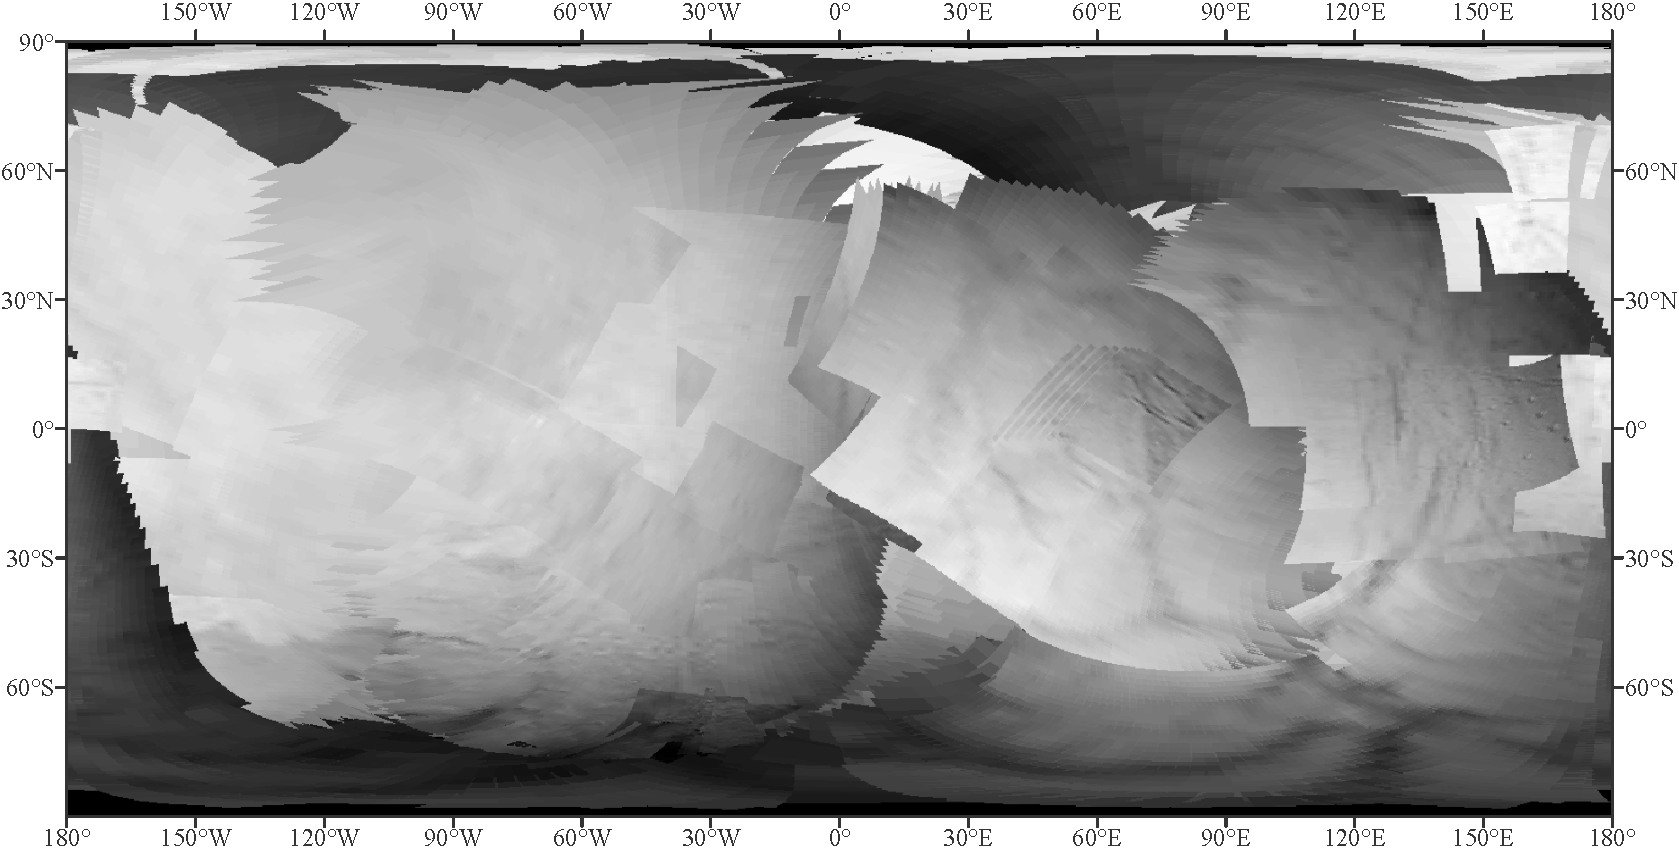
\includegraphics[width=.9\linewidth]{Fig_1}
%     \caption{}
%     \label{fig:}
% \end{figure}

% \begin{table}[!ht]
%     \caption{}
%     \label{tab:}
%     \begin{tabular}{l l r r}
%     \toprule
%     & & & \\
%     \midrule
%     & & & \\
%     \hline
%     \bottomrule
%     \end{tabular}
% \end{table}



\section{Conclusion}


% \end{linenumbers}

\clearpage

\section*{Acknowledgment}


\section*{Appendix A. Supplementary data}


\bibliography{biblio}

\end{document}